%
% Documento: Abordagem e modelagem do Problema
%

\chapter{Abordagem e Modelagem do Problema: Malhas de Controle}
\label{chap:abordagememdelo}
%Existem diversas maneiras de se implementar um sistema como este, tanto do ponto de vista do sistema distribuído e sua rede de comunicação, quanto do ponto de vista de controle e realimentação das malhas. Neste capítulo faz-se um detalhamento da abordagem do problema, do funcionamento do sistema como um todo e a modelagem escolhida para abordar os problemas. 

%Para resolução deste problema, primeiramente, estudou-se as possibilidades da implementação do mesmo em uma rede descentralizada, onde não tem-se um mestre definido, apenas uma sociedade de robôs que conforme precisam executar uma tarefa, vão recrutando e formando uma frota. No entanto, concluiu-se que, apesar de viável, a implementação de um sistema distribuído descentralizado seria muito complexo para ser abordado no período deste trabalho, que tem como objetivo principal o estudo de estratégias de controle de formação de múltiplos robôs móveis. Para tanto, foi adotada uma estrutura de rede centralizada denominada 'Mestre/Escravo' e um controle em cascata, utilizado para modularizar o problema e assim, tornar mais simples a implementação e o entendimento do mesmo. 

Como citado no \autoref{chap:Metod}, serão utilizadas duas abordagens diferentes, uma para resolver apenas o primeiro problema e a outra uma abordagem mais genérica que permite adaptação para resolução de ambos os problemas. A primeira abordagem, utilizará uma malha de controle de velocidade e uma malha de controle que será responsável pela comunicação entre os robôs e definirá a velocidade de cada robô, baseado na posição dos outros integrantes da frota.

Já a segunda abordagem, serão três malhas de controle: A primeira e mais interna será responsável pelo controle da velocidade angular de cada roda, para se chegar à posição (\emph{x,y}) desejada. A segunda, malha intermediária, será responsável para que cada robô chegue à um determinado ponto (\emph{x,y}) no espaço, portanto, será responsável por corrigir o posicionamento do robô. Ambas as malhas estarão presentes em cada um dos robôs da frota. A terceira malha, e portanto, a mais externa é responsável pela coordenação da frota, fornecendo a cada robô as informações necessárias para que o mesmo saiba o ponto (\emph{x,y}), onde deve ficar para consolidar e manter a formação.

Faz se então neste capítulo um detalhamento das malhas de controle utilizadas e das modificações realizadas para que a segunda abordagem atenda à ambos os problemas. Bem como, uma descrição de como funcionam as malhas responsáveis pela comunicação e pelo controle de formação para a resolução de cada um dos problemas e faz-se um levantamento dos possíveis problemas que podem surgir na implementação do sistema.   
%Faz-se então neste capítulo, primeiramente, a modelagem do problema, para que então, possa-se simular e implementar o problema. Para estabelecer o modelo matemático do problema, será considerado o modelo de robô mostrado na \autoref{fig:robo}.

\section{Malha de Controle 1: Velocidade Angular das Rodas}
\label{sec:malha1 } 
Como já dito anteriormente neste trabalho, este sistema de controle consiste em um controle de três malhas, e agora será abordado sobre a primeira malha. Ela controla os motores para atingir a velocidade angular desejada de cada roda ($\omega_{dr},\omega_{dl}$). Ou seja, a malha de controle vai receber a velocidade linear e angular que se deseja imprimir no robô e retornar a "potência" que deve ser aplicada a cada um dos motores para se atingir as velocidades desejadas. Como demonstrado pela /autoref{fig:malha1}.

\begin{figure}[!htb]
	\centering
	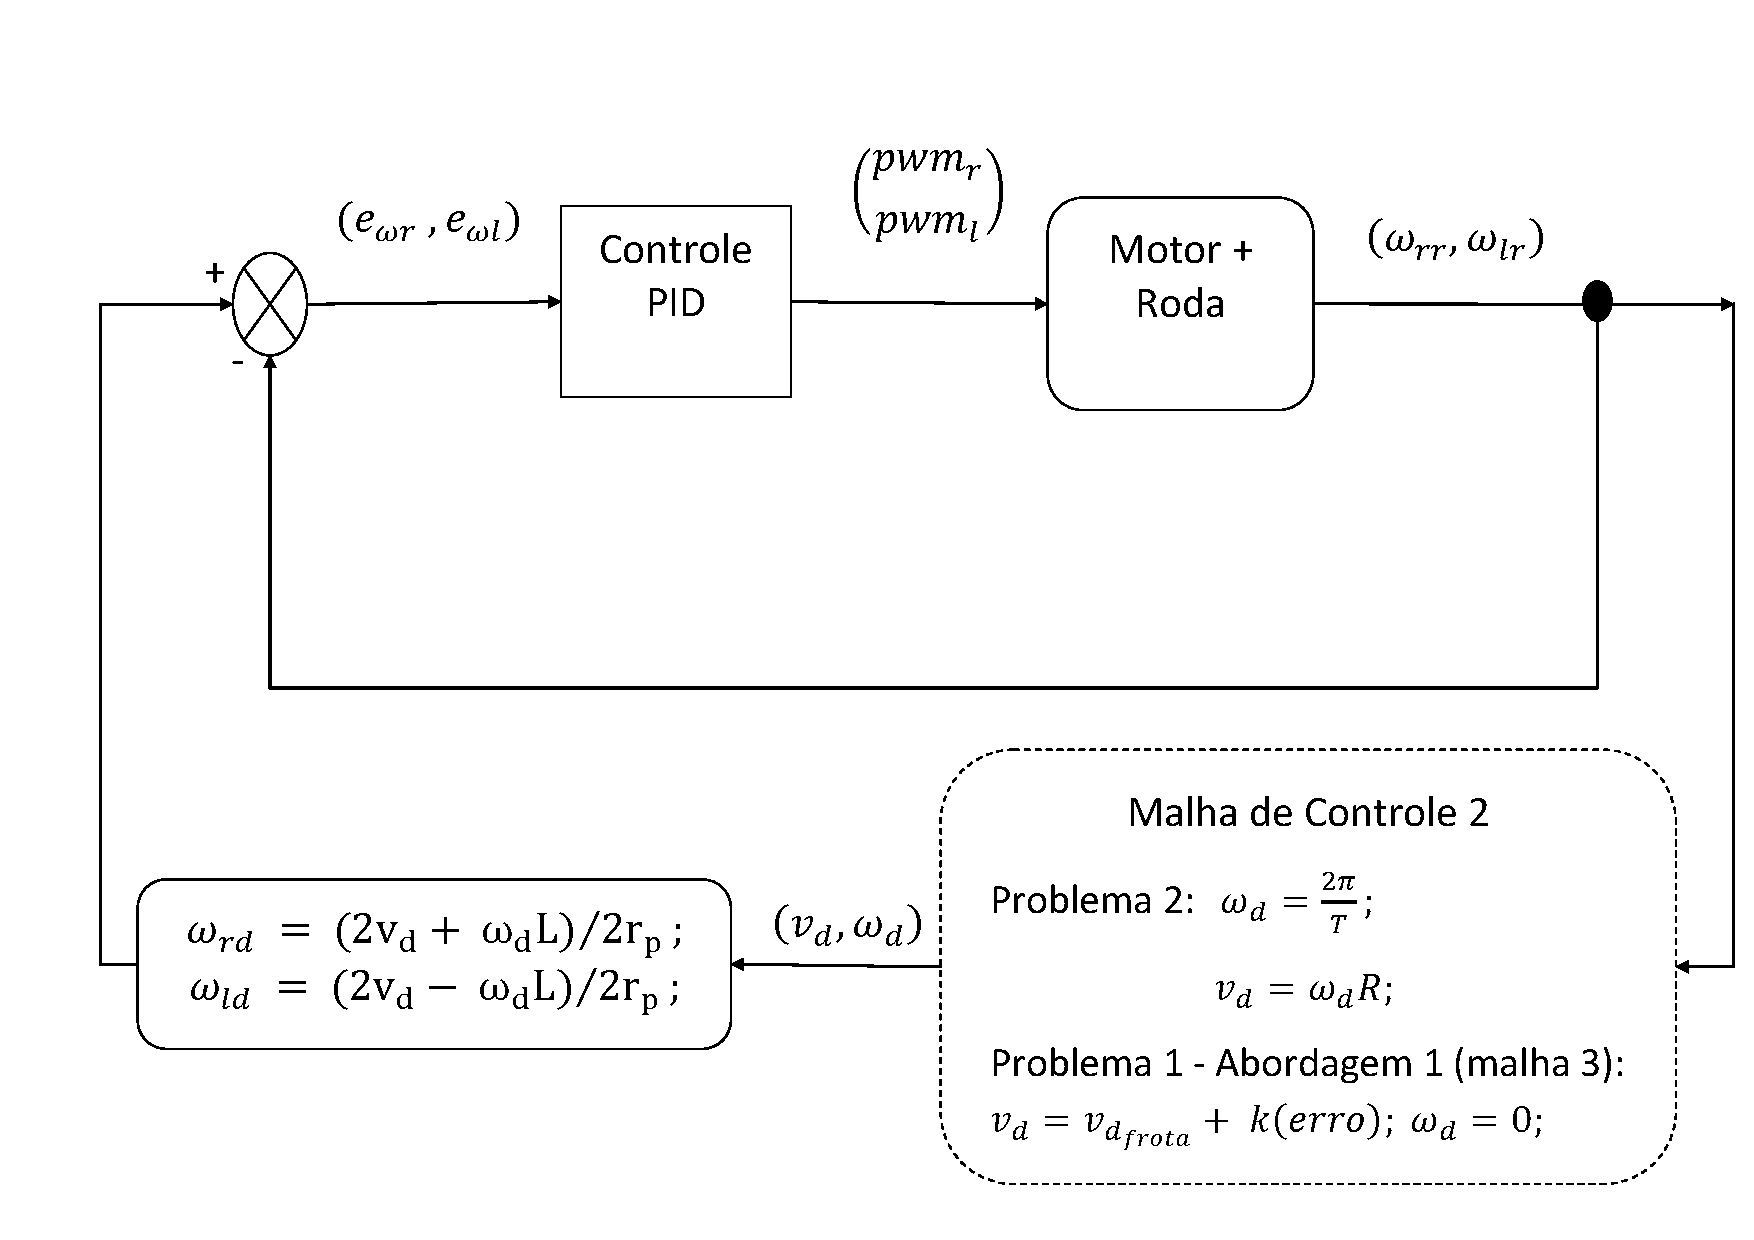
\includegraphics[width=1.0\textwidth]{./04-figuras/malha1}
	\caption{Primeira malha de Controle do Sistema - Controle da velocidade angular}
	\label{fig:malha1}
\end{figure}

É importante ressaltar que como o robô não é um elemento pontual\footnote{Veja a \autoref{fig:sistEst} para visualizá-lo como um elemento não pontual, que depende da variação de velocidade de cada roda para definir a velocidade e o sentido do robô.}, como considerado na \autoref{sec:modMatematico} ao descrever as equações do modelo, temos que descrever a velocidade angular (\emph{$\omega$}) e linear (\emph{$v$}) do robô em função de cada roda, para sabermos a potência a ser aplicada em cada uma delas para que o robô obtenha a velocidade e o sentido desejados.

A partir daí o módulo calcula velocidade angular desejada de cada roda, como demonstrado nas equações abaixo:
\begin{equation}
\omega_{dr} = \dfrac{2v + \omega_{d}L}{2r_{p}}	
\label{eq:velocangulardireita}
\end{equation} 
\begin{equation}
\omega_{dl} = \dfrac{2v - \omega_{d}L}{2r_{p}}	
\label{eq:velocangularesquerda}
\end{equation} 

onde:
\begin{itemize}
	\item $v_d$ é a velocidade linear desejada do robô ($m/s$);
	\item $\omega_{dr}$ é a velocidade angular desejada da roda direita ($rad/s$);
	\item $\omega_{dl}$ é a velocidade angular desejada da roda esquerda ($rad/s$);
	\item $r_{p}$ o raio do pneu ($m$);
	\item $L$ o tamanho do eixo do robô ($m$).	
\end{itemize}

Com a velocidade angular de cada roda  do robô, calculada através dos dados fornecidos pelos \emph{encoders}, é calculado o erro das velocidades, como mostrado nas equações abaixo, e o controlador os retorna as ações de controle que serão passadas como potência para cada uma das rodas.
\begin{equation}
e_{wr} = \omega_{dr} - \omega_{rr}
\label{eq:errVelAngDireita}
\end{equation} 
\begin{equation}
e_{wl} = \omega_{dl} - \omega_{rl}
\label{eq:errVelAngEsquerda}
\end{equation} 

onde:
\begin{itemize}
	\item $e_{wr}$ e $e_{wl}$ são os erros da velocidade angular da roda direita e esquerda, respectivamente;
	\item $\omega_{rr}$ é a velocidade angular real da roda direita e esquerda, respectivamente.
\end{itemize}	

\section{Malha de Controle 2: Posicionamento}
\label{sec:malha2 } 
Para que a malha de controle 3, que consiste no controle de formação da tropa funcione, primeiramente é necessário implementar o controle de posicionamento de cada robô. Ou seja, para que o robô cumpra a missão, é necessário que a malha de controle de formação passe para cada robô os parâmetros necessários para o ajuste da estrutura, tais como, posicionamento, velocidade e número de robôs da frota. Esse por sua vez, deve conseguir se posicionar na posição correta, recebida pela malha de controle 3,o que só será possível se a malha de controle 1 conseguir controlar adequadamente os motores para que eles imprimam a velocidade correta em cada roda.

Como pode ser visto na \autoref{fig:esq2}, o problema a ser resolvido pela segunda malha de controle, consiste em, dado um sistema de coordenadas cartesianas, onde têm-se um robô móvel de posição (\emph{$x_{r},y_{r}$}), cujo sentido (\emph{$\theta$}) é indicado pela sua variação dado o eixo \emph{x} do sistema, onde pretende-se fazer com que o robô chegue ao ponto desejado (\emph{$x_{d},y_{d}$}, recebido da malha de controle 3). Para tanto, a malha 2 funciona da seguinte maneira: Recebe da malha 3 os parâmetros necessários para o cálculo da posição desejada do robô (\emph{$x_{d},y_{d}$}), a partir daí é achado o erro de posição do robô (\emph{$e_{x},e_{y}$}), fazendo-se a diferença entre a posição desejada e a posição real do robô (\emph{$x_{r},y_{r}$}), que é obtida através dos \emph{encoders} do LEGO\textregistered, que se mostrou suficientemente precisos.

\begin{equation}
e_{r} = r_{d} - r_{r}
\label{eq:errr}
\end{equation}
\begin{equation}
e_{x} = x_{d} - x_{r}
\label{eq:errx}
\end{equation}
\begin{equation}
e_{y} = y_{d} - y_{r}
\label{eq:erry}
\end{equation}

Através do erro de posicionamento do robô, encontra-se o sentido desejado (\emph{$\theta_{d}$}), como mostrado na \autoref{eq:thetad}. Então, o erro de sentido do robô é obtido, através da \autoref{eq:errtheta} abaixo. 

\begin{equation}
\theta_{d} = \arctan(\dfrac{e_{y}}{e_{x}})
\label{eq:thetad}
\end{equation}
\begin{equation}
e_{\theta} = \theta_{d} - \theta_{r}
\label{eq:errtheta}
\end{equation}

O erro de sentido (\emph{$e_{\theta}$}) é passado para o controlador que retorna a velocidade linear e angular da ação de controle, que será passada para a malha mais interna. %Posteriormente, será feita uma comparação entre os controladores \emph{PI} e \emph{PID} e será definido o controlador a ser utilizado nesta malha.



\begin{figure}[!htb]
	\centering
	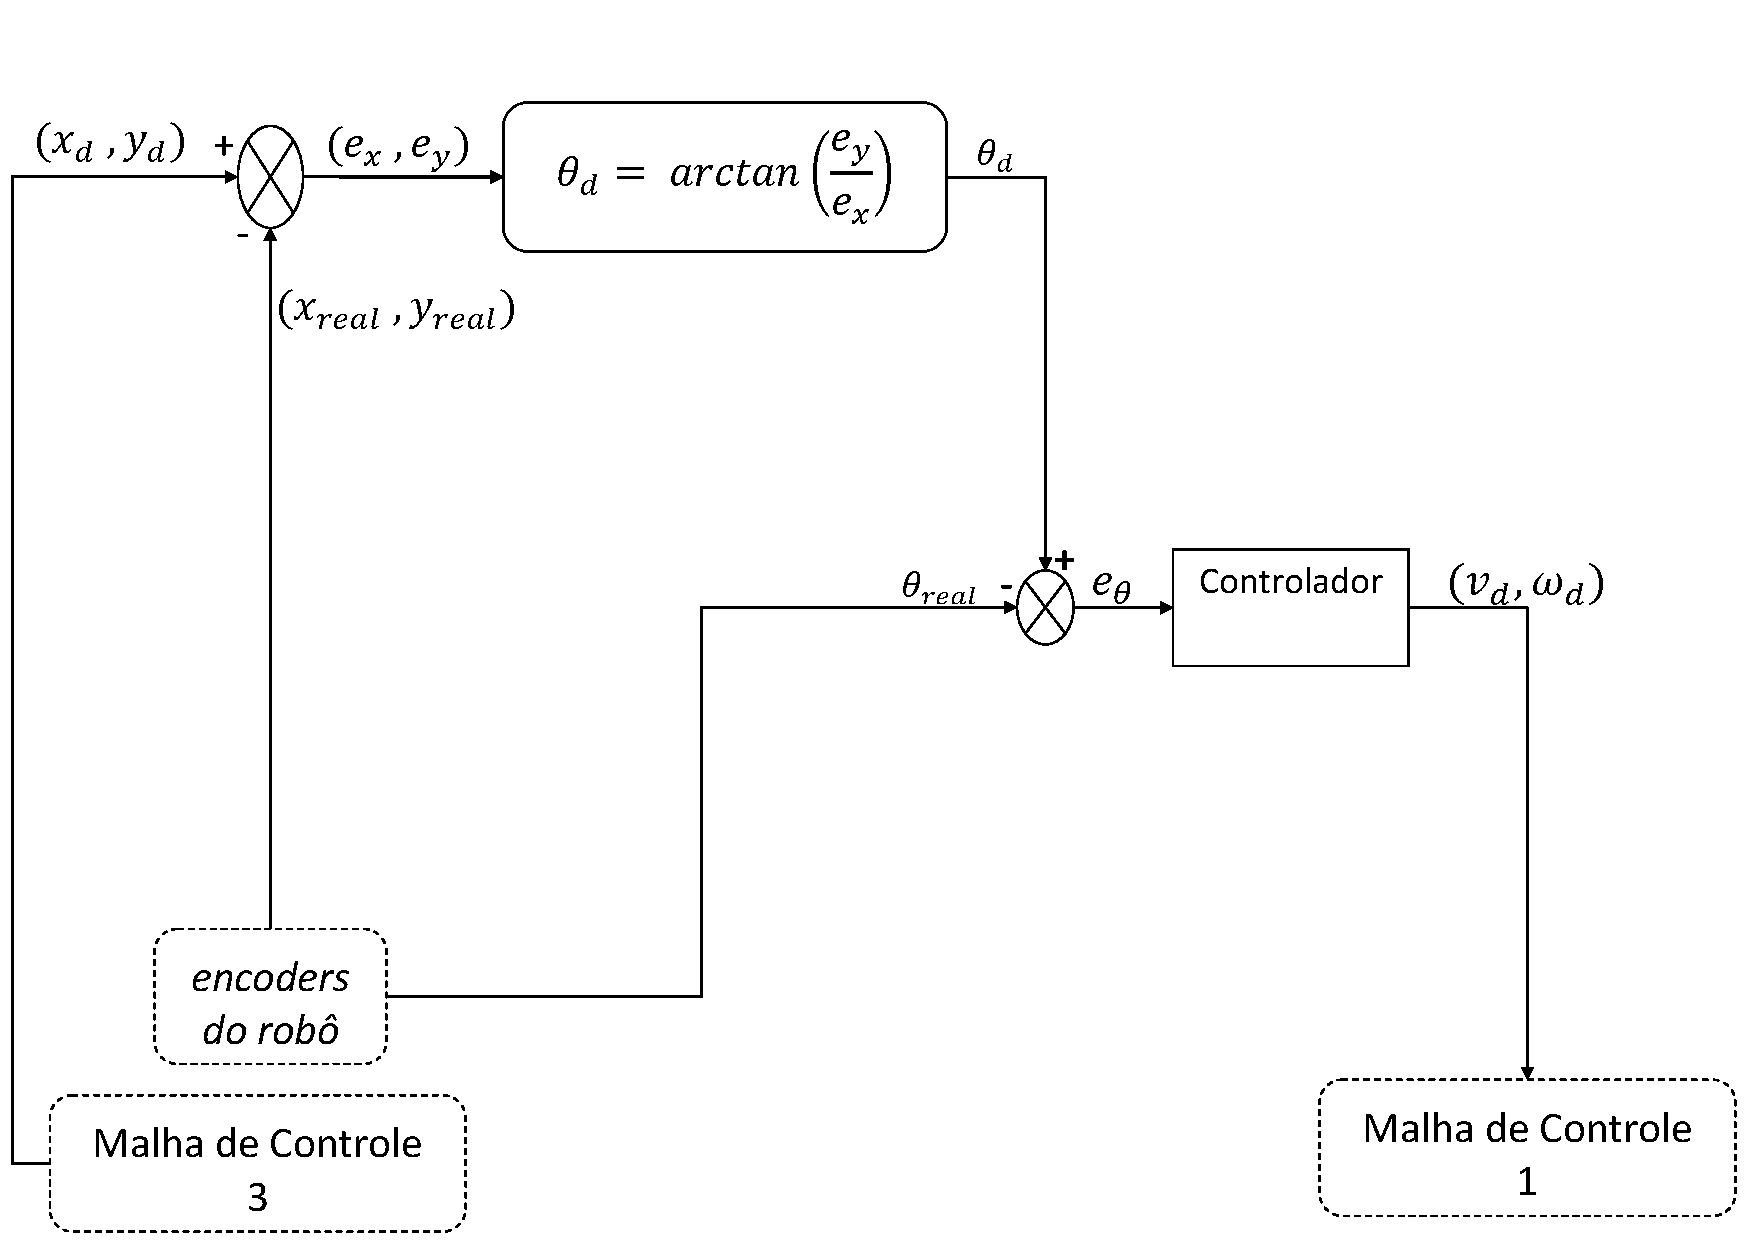
\includegraphics[width=1.0\textwidth]{./04-figuras/malha2}
	\caption{Segunda malha de Controle do Sistema - Controle de Posicionamento}
	\label{fig:malha2}
\end{figure}

\section{Malha de Controle 3: Controle de formação}
\label{sec:malha3 }









%Ou seja, deseja-se circular o alvo em um período de \emph{T} segundos, a malha de controle de velocidade vai receber a velocidade angular desejada ($ \omega _{d} $), que é uma derivação do período de circulação desejado, como mostrado na equação abaixo:

%Considerando que à medida que o sistema se estabiliza, o robô tende entra em movimento circular uniforme ao redor do alvo. Ou seja, a velocidade linear ($v$) tende a se igualar a velocidade angular ($\omega$) vezes o raio ($R$) de distância do alvo.

%\begin{equation}
%\omega = \dfrac{2\pi}{T}
%label{eq:velocangular}
%\end{equation}

%\begin{figure}[!htb]
%	\centering
%	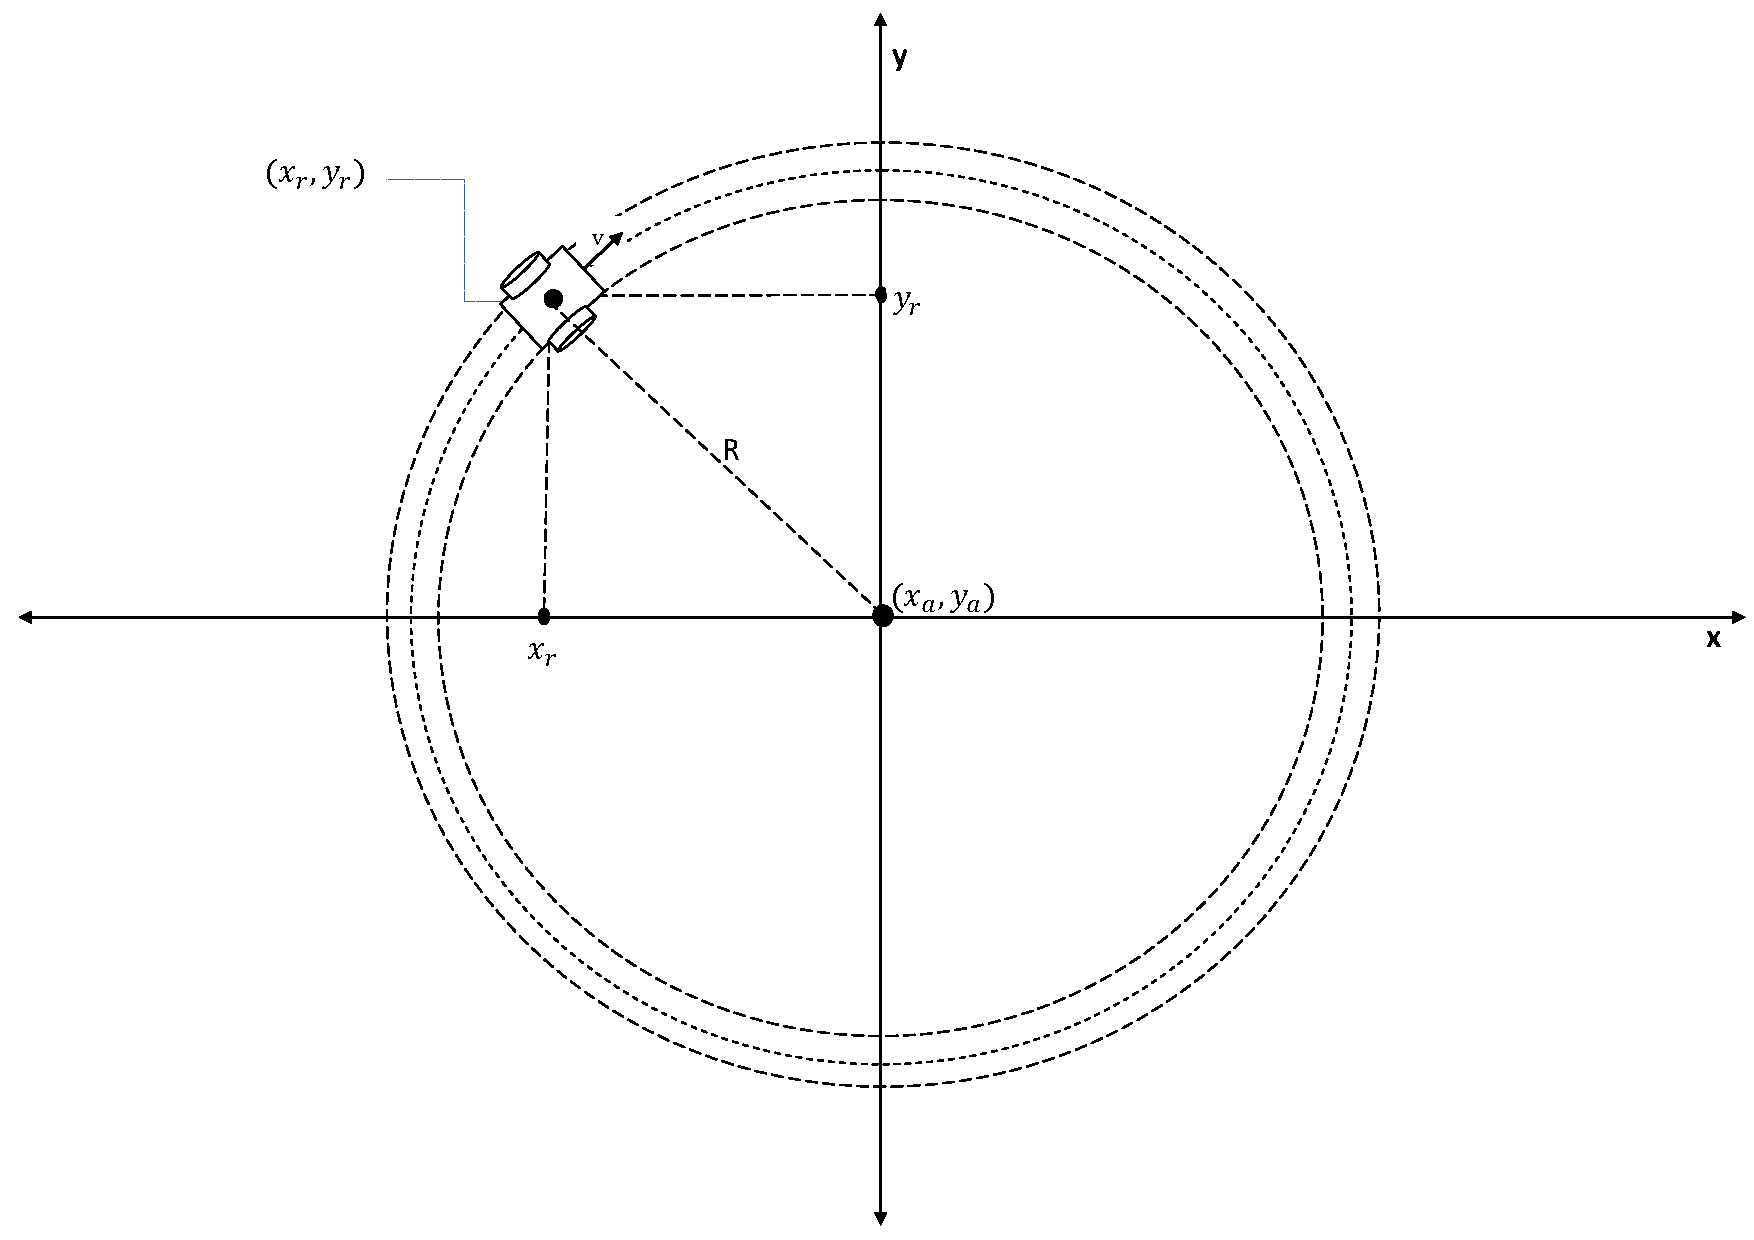
\includegraphics[width=1.0\textwidth]{./04-figuras/sistEstavel2}
%	\caption{Representação do sistema estável}
%	\label{fig:sistEst}
%\end{figure}

%\begin{figure}[!htb]
%	\centering
%	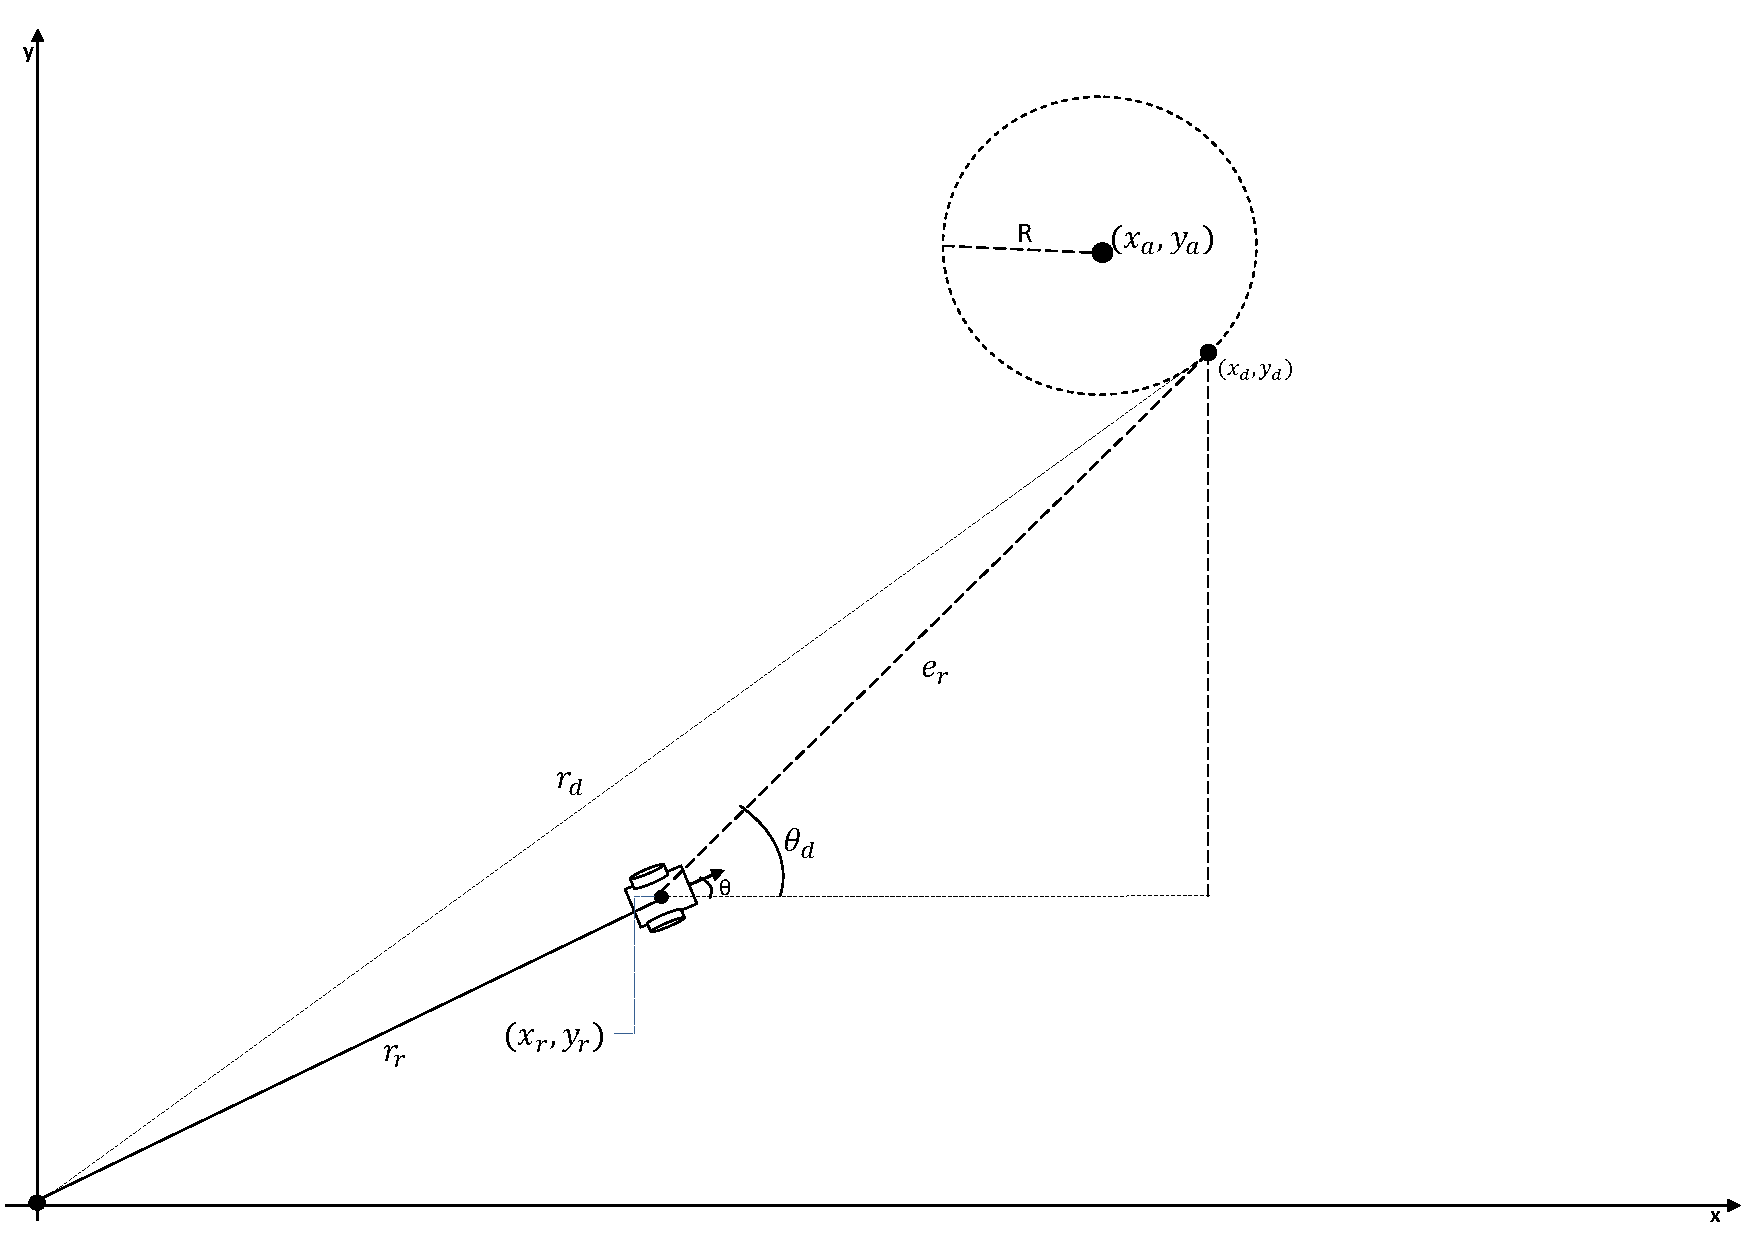
\includegraphics[width=1.0\textwidth]{./04-figuras/esqSistema}
%	\caption{Esquema do Sistema do Ponto de Vista de Apenas Um Agente}
%	\label{fig:esq2}
%\end{figure}


 

